\documentclass{article}%
\usepackage[T1]{fontenc}%
\usepackage[utf8]{inputenc}%
\usepackage{lmodern}%
\usepackage{textcomp}%
\usepackage{lastpage}%
\usepackage{graphicx}%
%
\usepackage{pgfplots}%
\pgfplotsset{compat=1.18}%
\title{Beam Analysis Report}%
\author{PyLaTeX Report Generator}%
\date{\today}%
%
\begin{document}%
\normalsize%
\maketitle%
\tableofcontents%
\newpage%
\section{Introduction}%
\label{sec:Introduction}%
This report presents a comprehensive analysis of beam loading and structural behavior.%


\begin{figure}[h!]%
\centering%
\includegraphics[width=0.8\textwidth]{C:/Users/DELL/Osdag/fossee-osdag-pylatex-report/src/assets/sample_beam.png}%
\caption{Simply supported beam under loading}%
\end{figure}

%
\section{Load Data}%
\label{sec:LoadData}%
\begin{tabular}{|c|c|c|}%
\hline%
\textbf{x (m)}&\textbf{Shear Force (N)}&\textbf{Bending Moment (Nm)}\\%
\hline%
0.0&45.0&0.0\\%
\hline%
1.5&36.0&60.75\\%
\hline%
3.0&27.0&108.0\\%
\hline%
4.5&18.0&141.75\\%
\hline%
6.0&9.0&162.0\\%
\hline%
7.5&0.0&168.75\\%
\hline%
9.0&{-}9.0&162.0\\%
\hline%
10.5&{-}18.0&141.75\\%
\hline%
12.0&27.0&108.0\\%
\hline%
13.5&{-}36.0&60.75\\%
\hline%
15.0&{-}45.0&0.0\\%
\hline%
\end{tabular}

%
\section{Analysis}%
\label{sec:Analysis}%

\begin{center}
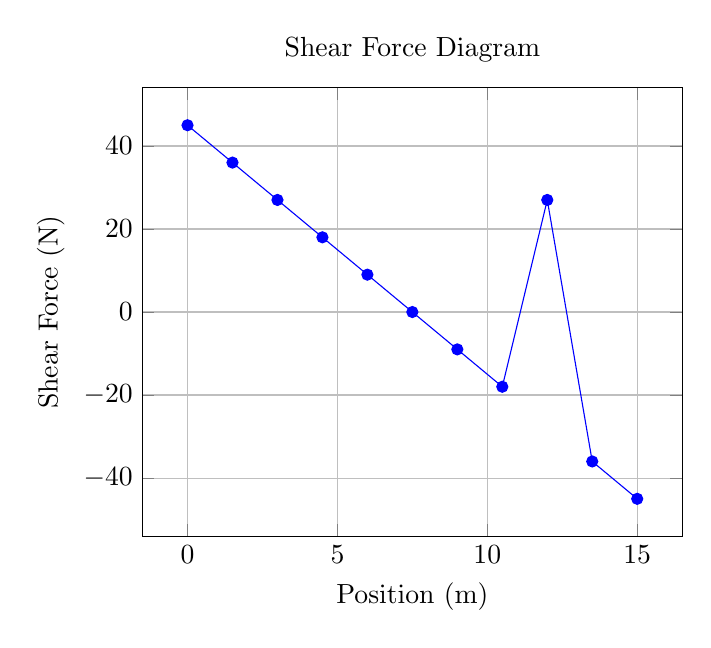
\begin{tikzpicture}
  \begin{axis}[title={Shear Force Diagram},xlabel=Position (m),ylabel=Shear Force (N),grid=both]
    \addplot[color=blue,mark=*] coordinates {
    (0.0,45) (1.5,36) (3.0,27) (4.5,18) (6.0,9) (7.5,0) (9.0,-9) (10.5,-18) (12.0,27) (13.5,-36) (15.0,-45)
    };
  \end{axis}
\end{tikzpicture}
\end{center}
%

\begin{center}
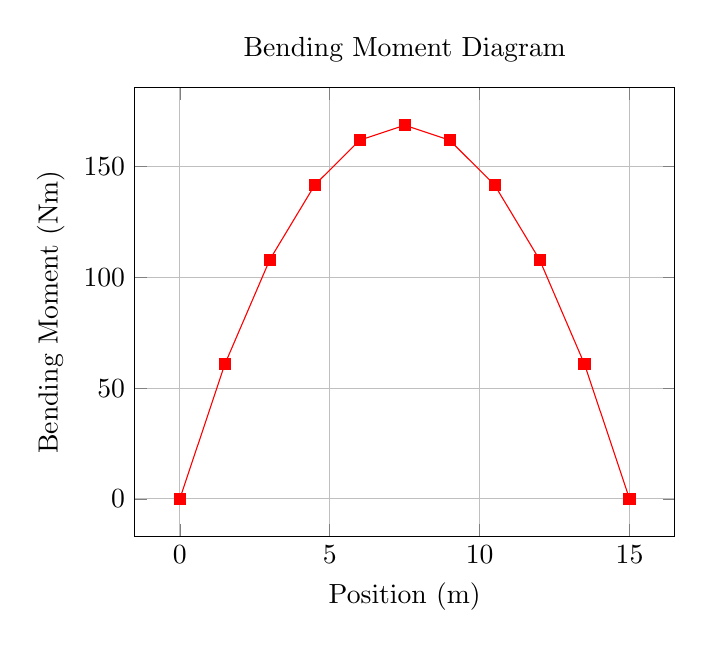
\begin{tikzpicture}
  \begin{axis}[title={Bending Moment Diagram},xlabel=Position (m),ylabel=Bending Moment (Nm),grid=both]
    \addplot[color=red,mark=square*] coordinates {
    (0.0,0.0) (1.5,60.75) (3.0,108.0) (4.5,141.75) (6.0,162.0) (7.5,168.75) (9.0,162.0) (10.5,141.75) (12.0,108.0) (13.5,60.75) (15.0,0.0)
    };
  \end{axis}
\end{tikzpicture}
\end{center}

%
\end{document}